\documentclass[a4paper,twoside,master.tex]{subfiles}
\begin{document}
\lecture{39}{Friday, November 15, 2019}{Continuum Limit of Harmonic Chain}

Allow me to restate the Hamiltonian, dropping the harmonic oscillator part, which isn't physical in real atomic structures:
\begin{equation}
    \vu{H} = \sum_j (\frac{1}{2} m \dot{x}^2_j + \frac{1}{2} m \omega_1^2 (x_{j+1} - x_j)^2
\end{equation}
and
\begin{equation}
    \Omega(k) = 2 \omega_1 \abs{\sin(\frac{kl}{2})} = (\omega_1 l)k
\end{equation}
where $ m \omega_1^2 $ is the strength of the atomic bond, roughly modeled as a spring.

When we go to the continuum limit, our discrete sum becomes an integral $ \sim \int \frac{\dd{x}}{l} $. Now our discrete $ x_j $ should also be replaced by some continuous function $ u(x) $, so $ x_{j+1} - x_j \approx l \pdv{u(x)}{x} $. If $ k $ corresponds to a length scale much larger than the size of the atoms, we no longer care about the mass of the atoms, but rather the mass density $ \mu = \frac{m}{l} $. Of course, $ \dot{x}_j \to \pdv{u(x)}{t} $ and we will assign a new variable $ m \omega_1^2 l^2 \to K $ such that $ \omega_1 = \sqrt{\frac{K}{\mu}} - l $. $ K $ is an elastic constant.

\begin{equation}
    H = \int \dd{x} \left\{ \frac{1}{2} \mu \left( \pdv{u}{t} \right)^2 + \frac{1}{2} K \left( \pdv{u}{x} \right)^2 \right\}
\end{equation}

Solutions to this equation are
\begin{equation}
    u_{k}(x,t) = A e^{\imath (k x - \omega t)} 
\end{equation}
where $ \omega = vk $ with $ v = \sqrt{\frac{K}{\mu}} $.

As $ l $ grows smaller, $ \frac{\pi}{l} $ grows bigger\textemdash the Brillouin zone gets larger, and the dispersion relation grow as shown in \Cref{fig:dispersion_relation_continuum}.

\begin{figure}[h]
    \centering
    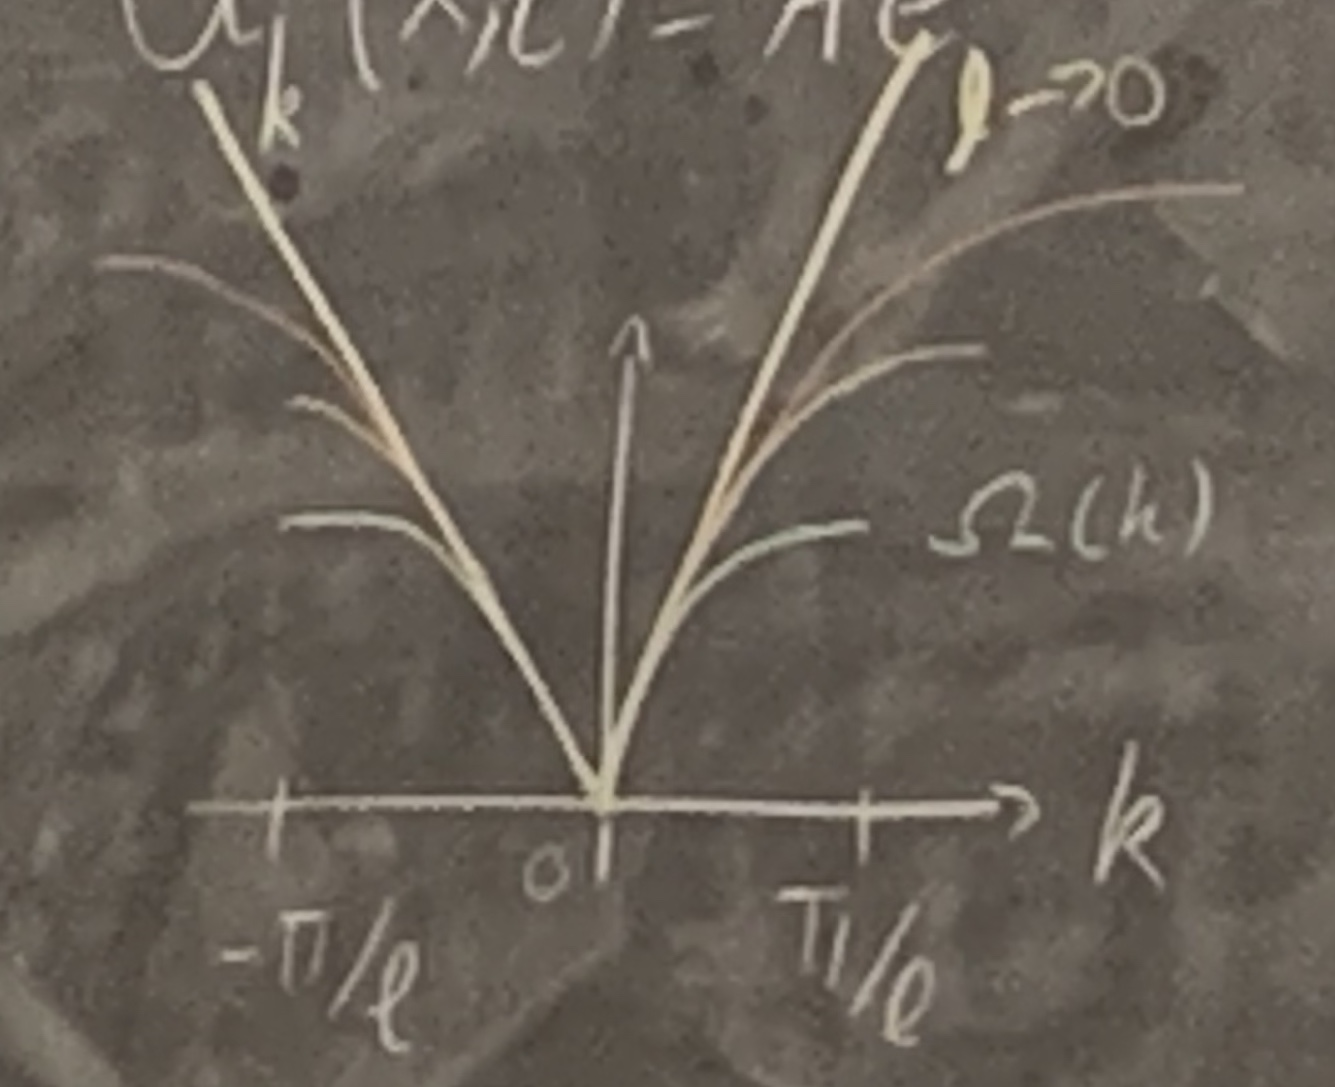
\includegraphics[width=\textwidth/2]{figures/lec_39_dispersion_relation.jpg}
    \caption{Dispersion relation as $ l \to 0 $}
    \label{fig:dispersion_relation_continuum}
\end{figure}

\section{Blackbody Radiation}
\label{sec:blackbody_radiation}

Think of a blackbody as a box of photons. Photons are allowed to leave (radiate) if they are excited.

Say we have a 1-D box which ranges from $ [0,L] $ with boundary conditions where the field vanishes at the boundaries. We see that the set of wavenumbers which conform to these conditions are $ k_j = \frac{\pi}{L} j $ and the allowed frequencies are $ \omega_j = ck_j $. Call the density of states $ D(\omega) $ and we can define the number of states in an interval $ (\omega, \omega + \dd{\omega}) $ as $ D(\omega) \dd{\omega} $. The number of modes with frequency less than $\omega$ is $ \mathscr{N}(\omega) = \frac{L \omega}{\pi c} $. Therefore,
\begin{equation}
    D(\omega) = \dv{\mathscr{N}}{\omega} = \frac{L}{\pi c}
\end{equation}

In 3-D,
\begin{equation}
    \mathscr{N}(\omega) = \frac{4 \pi}{3} \left( \frac{\omega L}{2 \pi c} \right)^3
\end{equation}

The values of allowed $ k $ form a discretely spaced set. If we then choose an $\omega$, we can see how many $ k $ values lie in the dispersion band for a particular $\omega$ (again, see \Cref{fig:dispersion_relation_continuum}).

For photons in 3-D space, we actually need to multiply this value by two, since we can have two different polarized states:

\begin{equation}
    \mathscr{N}(\omega) = \frac{4 \pi}{3} \left( \frac{\omega L}{2 \pi c} \right)^3 \times 2
\end{equation}

Given this $ \mathscr{N} $,
\begin{equation}
    D(\omega) = \frac{\omega^2}{\pi^2} \frac{1}{c^3} V
\end{equation}
where $ V $ is the volume of the box.

Recall from this morning we discussed the expectation value of the Hamiltonian for a particular temperature and value of $\omega$:
\begin{equation}
    \vu{H} = \int \dd{k} \vu{H}(k)
\end{equation}
so
\begin{equation}
    \ev{ \vu{H}}(\omega) - \frac{1}{2} \hbar \omega = \frac{\omega^2}{\pi^2} \frac{1}{c^3} V \frac{\hbar \omega}{e^{\frac{\hbar \omega}{kT}} - 1} 
\end{equation}
because many of the modes in the 3-D box are degenerate (just in different directions). The spectral energy density is the famous blackbody spectrum (see \Cref{fig:blackbody_spectrum})

\begin{figure}[h]
    \centering
    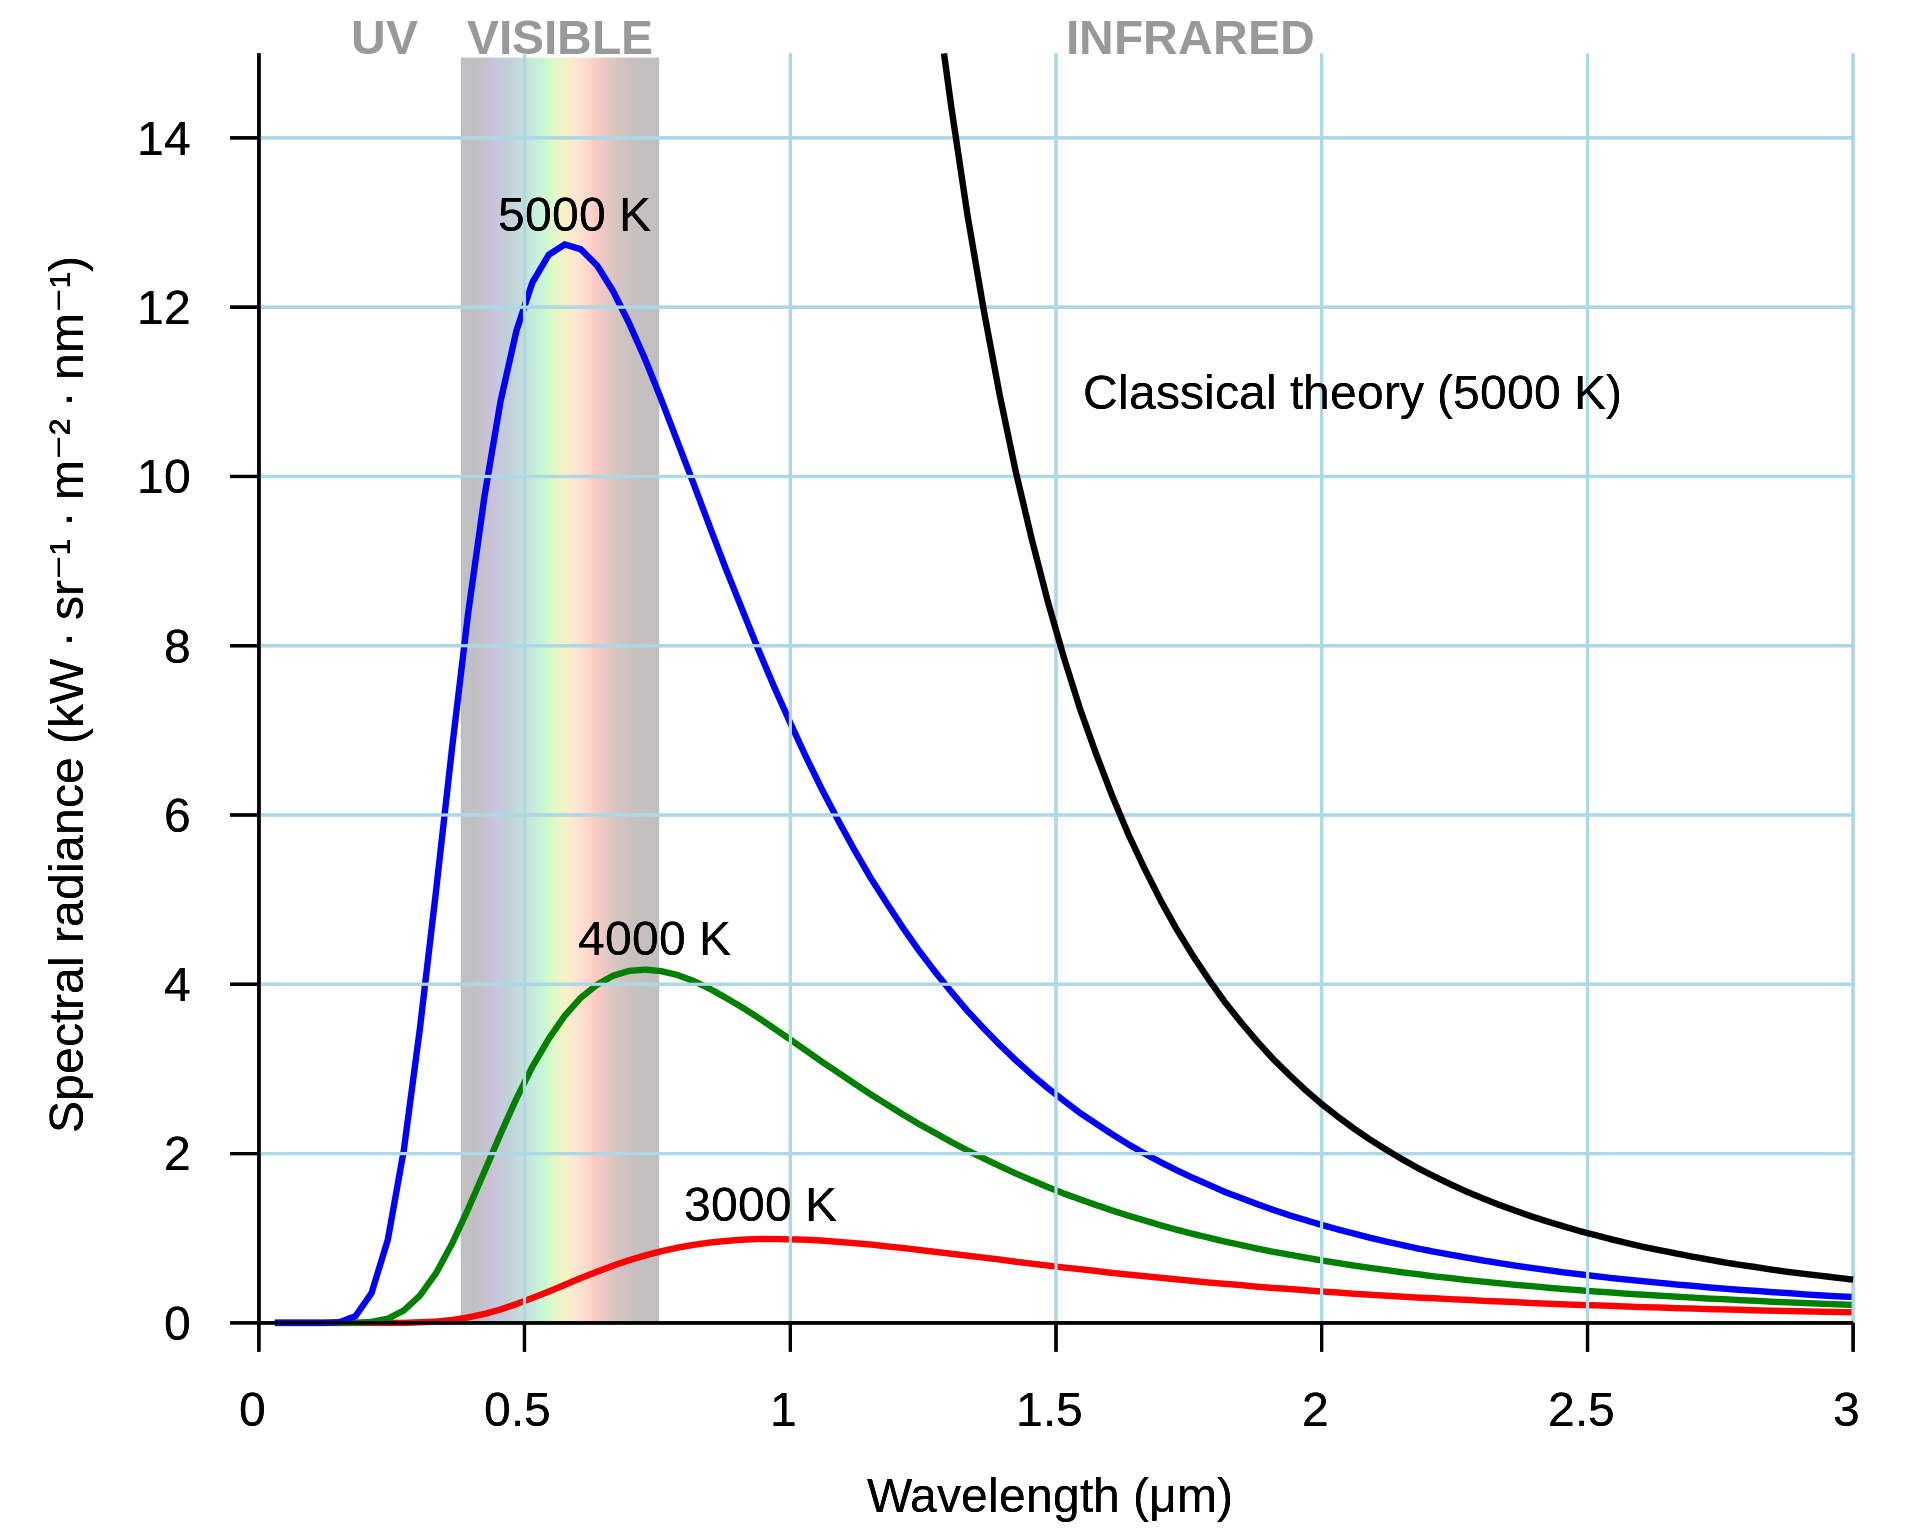
\includegraphics[width=\textwidth/2]{figures/lec_39_blackbody_spectrum.png}
    \caption{The Blackbody Energy Density Spectrum}
    \label{fig:blackbody_spectrum}
\end{figure}

We can see that the spectrum increases with $ \omega^2 T $ at low $ \omega $, but at some point ($\omega = \frac{kT}{\hbar}$ ) we leave this Classical behavior and the spectrum changes like $ e^{-\frac{\hbar \omega}{kT}} $.

\section{Heat Capacity}
\label{sec:heat_capacity}

We can describe a characteristic called heat capacity which corresponds to the way the heat contained in an object changes with temperature:
\begin{equation}
    C_v = \pdv{U(T)}{T}
\end{equation}

For a harmonic solid (something with quadratic terms in the Hamiltonian, no higher-order terms), the total energy constant is proportional to the total number of atoms present and the average amount of energy per atom:
\begin{equation}
    U = 3N\ev{\vu{H}}
\end{equation}

Note that phonon modes have three polarizations (degenerate eigenstates in 3-D). Let's examine the Einstein model, where the density of states is described by
\begin{equation}
    D(\omega) = 3N \delta(\omega - \omega_E)
\end{equation}
This is equivalent to bringing back the local harmonic oscillators which we threw a way in the continuum limit, and it removes the interaction between nearby atoms. It's not a great model. For this model,
\begin{equation}
    C_v \sim e^{- \frac{\hbar \omega_E}{k_B T}}, \quad T \to 0 
\end{equation}
This explains nicely why heat capacity vanishes at low $ T $ and approaches $ 3 k_B $ as $ T \to \infty $, the Classical limit. The Classical (high temp) and quantum (low temp) regions are separated by characteristic temperature $ \frac{\hbar \omega_E}{k_B} $.

There is another model by Debye which takes into account the low frequency modes:
\begin{equation}
    D(\omega) = \frac{\omega^2}{\pi^2} \frac{1}{c^3} V \divisionsymbol 2 \times 3
\end{equation}
Note that $ c $ here is the speed of sound, not light.

We divide by $ 2 $ to eliminate the degeneracy of photon polarizations which was present in the blackbody derivation, but multiply by $ 3 $ to reintroduce the degeneracy of the phonon states.

While both models behave the same way in their extremes, the Debye model varies like $ T^3 $ at low temperatures while Einstein's model varies like  $ e^{- \frac{\hbar \omega_E}{kT}} $.

\end{document}
